% ============================================================================
%  Mitigating Smart-Charging Rebound Peaks Under Network-Aware Dynamic
%  Pricing on Low-Voltage Feeders
%  IEEE PES General Meeting 2027 -- conference paper, 5-page limit
%
%  Build:   pdflatex paper.tex (twice). Needs IEEEtran.cls (in TeX Live and
%           Overleaf). Put the six figures (PDF or PNG) in a folder called figures/
%           next to this file (../figures/ also works inside the repo).
%           Table II is typed in below; scripts/make_tables.py writes the same
%           rows to results/table_main.tex if the results are regenerated.
% ============================================================================

\documentclass[conference]{IEEEtran}
\IEEEoverridecommandlockouts

\usepackage{cite}
\usepackage{amsmath,amssymb,amsfonts}
\usepackage{algorithmic}
\usepackage{algorithm}
\usepackage{graphicx}
\usepackage{textcomp}
\usepackage{booktabs}
\usepackage{url}
\usepackage[hidelinks]{hyperref}
\usepackage{tikz}
\usetikzlibrary{arrows.meta,positioning}

\graphicspath{{figures/}{../figures/}}

\newcommand{\pkwh}{\,p/kWh}
\newcommand{\CVaR}{\mathrm{CVaR}}
\setlength{\aboverulesep}{0.3ex}
\setlength{\belowrulesep}{0.4ex}

\begin{document}

\title{Mitigating Smart-Charging Rebound Peaks\\Under
Network-Aware Dynamic Pricing on Low-Voltage Feeders}

\author{\IEEEauthorblockN{Anay Gupta}
\IEEEauthorblockA{\textit{Dept. of Electrical and Electronic Engineering} \\
\textit{Imperial College London}\\
London, United Kingdom \\
anay.gupta25@imperial.ac.uk}
}

\maketitle

% ============================================================== ABSTRACT
\begin{abstract}
The rapid adoption of electric vehicles (EVs) challenges low-voltage
networks. A home charger draws as much power as several
households, so many vehicles charging at once can overload the street's
feeder. Time-of-use tariffs move charging away from
the evening peak, but every driver sees the same cheap period, creating a
rebound peak when it begins. Network-aware tariffs avoid this by pricing each
half-hour from the feeder's spare capacity, assuming drivers respond
differently. Smart chargers do not: they run similar algorithms on the
same price, so they all choose the same cheapest half-hours. This research
models such chargers, including a commercial scheduler, on a 75-home London
feeder using Monte Carlo simulation, and tests three mitigations:
a random start delay, a household-specific price offset (a dither) and a cap
on EV power per half-hour (a quota). At full EV ownership, every shared
price raised the 95\% conditional value at risk of the daily peak from
129~kW to 147--151~kW. The delay left 36\% of days over the 100.9~kW limit, a
$\pm$2\pkwh{} dither 7.0\% and a quota 5.5\%. The dither suffices up to 80\%
EV ownership; beyond that, a quota is needed.
\end{abstract}

\begin{IEEEkeywords}
Demand response, distribution networks, dynamic pricing, electric vehicle
charging, rebound effect, smart charging.
\end{IEEEkeywords}

% ============================================================== INTRODUCTION
\section{Introduction}

The homes on a street are supplied by one low-voltage (LV) cable, called a
feeder, whose limit is set for ordinary household demand. On the London
feeder studied here, 75 homes draw about 1~kW each at the evening peak,
against a limit of 100.9~kW \cite{gupta2027}. A home EV charger draws
7.4~kW, as much as about seven homes, so the spare capacity is used up by
only three cars. When more cars than that charge at once, demand breaches the
limit, and the cables and transformer overheat or trip
\cite{gupta2027,crozier2020}.

\begin{figure}[t]
\centering
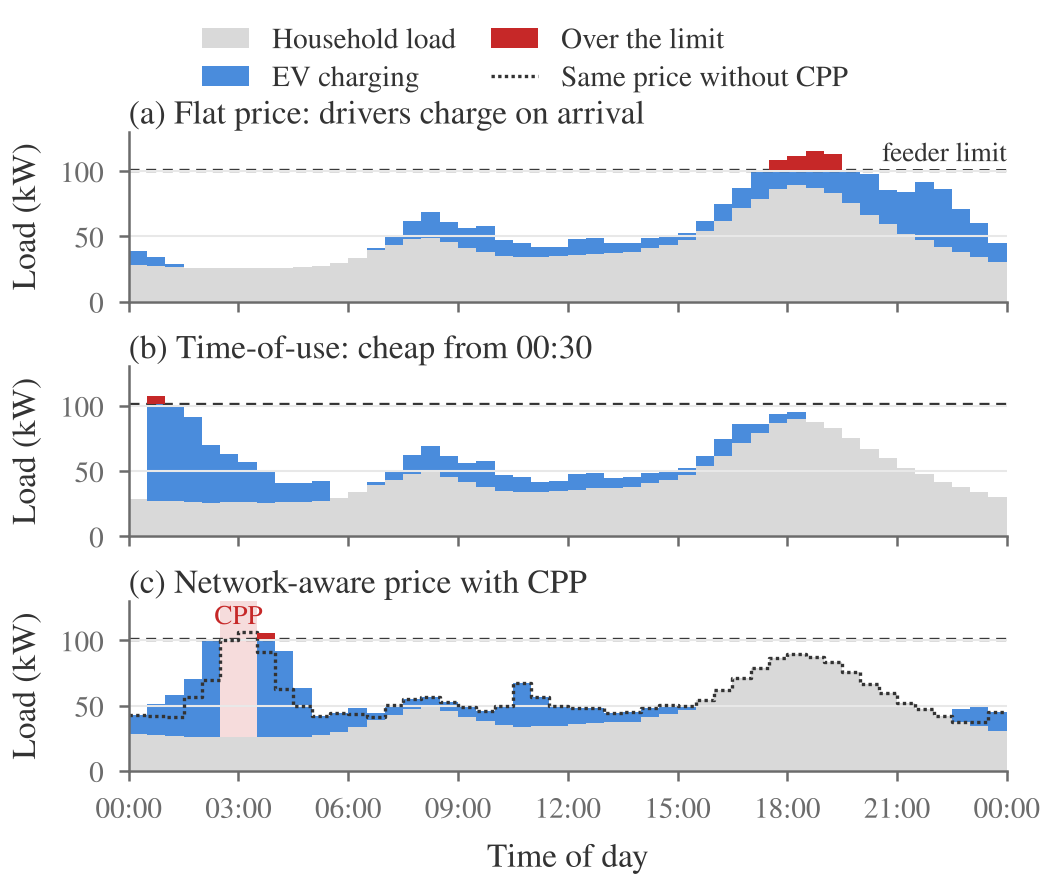
\includegraphics[width=\columnwidth]{f1_problem}
\caption{Half-hourly load on one cold weekday on the studied London feeder,
with EVs in 80\% of homes and every charger responding to the price. (a)
Uncontrolled charging adds to the evening peak. (b) A time-of-use tariff
starts every charger at 00:30. (c) The network-aware price moves charging to
around 03:00; its CPP empties 02:30--03:30, and the chargers all restart when
it ends.}
\label{fig:problem}
\end{figure}

Fig.~\ref{fig:problem}(a) shows that the problem is the evening: drivers plug
in when they get home, just as household demand peaks. Overnight, the same
feeder has room for about ten chargers, and most cars stay plugged in until
morning, so moving charging into this trough would deliver the same energy
within the limit. A time-of-use (ToU) tariff such as Octopus Go, cheap from
00:30 to 05:30 \cite{octopus}, aims to do this. But every driver sees the
same cheap window, so demand for its first half-hour jumps: on this day 11
chargers switched on together at 00:30, and the feeder went over its limit
again (Fig.~\ref{fig:problem}(b)). This is a \emph{rebound peak}, a new peak
created by the price signal itself.

Our earlier network-aware tariff avoids a single cheap window
\cite{gupta2027}. It prices each half-hour from the feeder's spare capacity,
adds a critical-peak price (CPP), a surcharge high enough to stop charging,
wherever forecast EV demand would use more than 80\% of that capacity, and
recomputes the price and the demand it creates until the two agree
(fixed-point iteration). This relies on drivers responding differently. Wen
\emph{et al.} \cite{wen} found that about 20\% of drivers respond strongly
to charging prices, 60\% respond slightly, and 20\% hardly respond at all,
so the demand that moves is spread over several half-hours.

Smart chargers remove this spread. New home chargers must now be smart
\cite{scpregs}: a scheduling algorithm reads the next day's prices and books
the cheapest half-hours before the car is needed \cite{evenergy}. Every
charger on the street runs a similar algorithm on the same price, so all of
them choose the same half-hours. Trials already show the effect: network
studies driven by charging data from 96 smart-charging homes on a ToU tariff
found a new overnight peak that exceeds the evening peak once about 30\% of
homes have an EV \cite{samende2025}, and data from 854 homes show a sharp
spike at 00:30, when the cheap rate begins \cite{catapult2025}. Fig.~\ref{fig:problem}(c) shows three
consequences for the network-aware tariff.
\emph{Demand for the cheapest half-hours rises}: without the CPP, the feeder
reaches 106~kW at 03:00. \emph{The CPP moves the peak rather than spreading
it}: the next cheapest half-hour is the same for every charger, so they all
wait for the surcharge to end and switch on in the same minute (11 chargers
at 03:30). \emph{The price never settles}: demand leaves whichever half-hour
the CPP covers, so the CPP keeps following it. The mandated random start
delay of up to 10~minutes \cite{scpregs} staggers switch-ons, but leaves the
cars in the same half-hour.

Since every charger makes the same decision, a fix must either give the
chargers different decisions or limit how many can act on one. We test three
on the network-aware tariff: the random delay; a \emph{price dither}, which
adds a small household-specific offset of up to $\pm$2\pkwh{} so that
households have different cheapest half-hours; and a \emph{quota}, which caps
EV power in each half-hour and lets chargers book it in order of price. Our
contributions are:
\begin{enumerate}
\item We show that when every charger is smart, a network-aware tariff makes
the worst days worse than uncontrolled charging, its CPP never settles, and
the CPP nearly doubles the chargers switching on together. Herding has been
simulated for wholesale prices \cite{hein2026}; we show it for a
network-aware tariff, minute by minute.
\item We test the random delay that chargers must already apply, which to
our knowledge has not been done before, against a household price dither,
adapted from the randomised group prices of \cite{flath2016}, and a quota,
similar to operating envelopes that limit each home's power draw
\cite{fani2024}.
\item We show that this holds for a commercial scheduler, and that mixing
vendors' schedulers does not help a network-aware price, because it leaves
no ties to break. All code and data are public\footnote{Code and data:
\url{https://github.com/RISKMASTER16/evalgopricing}.}.
\end{enumerate}

% ============================================================== MODEL
\section{Model}
\label{sec:model}

\begin{figure}[t]
\centering
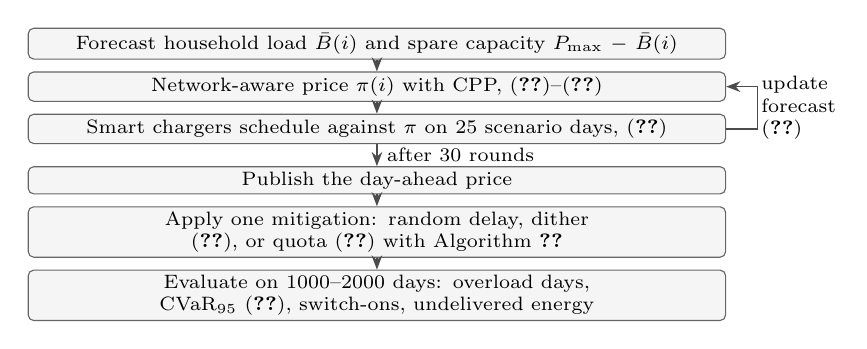
\begin{tikzpicture}[
  font=\scriptsize, node distance=1.5mm,
  box/.style={draw=black!60, rounded corners=2pt, fill=black!4, align=center,
              text width=0.72\columnwidth, inner sep=1.8pt},
  ar/.style={-{Stealth[length=1.8mm]}, semithick, draw=black!70}]
\node[box] (bg)  {Forecast household load $\bar{B}(i)$ and spare capacity
  $P_{\max} - \bar{B}(i)$};
\node[box, below=of bg] (pr) {Network-aware price $\pi(i)$ with CPP,
  \eqref{eq:network}--\eqref{eq:cpp}};
\node[box, below=of pr] (sim) {Smart chargers schedule against $\pi$ on 25
  scenario days, \eqref{eq:smart}};
\node[box, below=2.8mm of sim] (pub) {Publish the day-ahead price};
\node[box, below=of pub] (mit) {Apply one mitigation: random delay, dither
  \eqref{eq:dither}, or quota \eqref{eq:quota} with Algorithm~\ref{alg:quota}};
\node[box, below=of mit] (ev) {Evaluate on 1000--2000 days: overload days,
  $\CVaR_{95}$ \eqref{eq:cvar}, switch-ons, undelivered energy};
\draw[ar] (bg) -- (pr);
\draw[ar] (pr) -- (sim);
\draw[ar] (sim) -- node[right, font=\scriptsize]{after 30 rounds} (pub);
\draw[ar] (pub) -- (mit);
\draw[ar] (mit) -- (ev);
\draw[ar] (sim.east) -- ++(4mm,0) |- node[pos=0.25, right, align=left,
  font=\scriptsize, inner sep=1pt]{update\\forecast\\\eqref{eq:fp}} (pr.east);
\end{tikzpicture}
\caption{The method. The price is recomputed against the charging it creates;
each mitigation is then applied and evaluated on the same simulated days.}
\label{fig:method}
\end{figure}

\subsection{Demand and background load}

Fig.~\ref{fig:method} summarises the method. EV demand uses the
session-level Monte Carlo model of \cite{gupta2027}. Each
day, a feeder with $n_{\text{EV}}$ cars has $\mathrm{Poisson}(n_{\text{EV}}k)$
home-charging sessions, where $k$ is the average number of sessions per car
per day. Each session draws a daily distance $s$, an arrival state of charge
and a plug-in time, and requests $E = (1-\mathrm{SOC})\,s\,W_{100}/(100k)$,
capped by the battery size. We add two things. First, each session has a
departure time. Cars plugged in between 14:00 and 04:00 leave
the next morning at $\mathcal{N}(07{:}30,1\,\text{h})$, and daytime plug-ins
stay for 3--8~h. Requests are trimmed to what a 7.4~kW charger can deliver
before departure, so any energy left undelivered is caused by the mitigation,
not by the request. Second, the model runs in one-minute steps, because
chargers that switch on together do so within minutes. Non-EV load is a
half-hourly forecast profile scaled by a lognormal day factor with a
coefficient of variation of 0.10, which is the operator's main forecast error.

\subsection{Smart and legacy chargers}

A share $s$ of chargers is smart. A smart charger with plug-in time $a$,
departure time $b$ and price $\pi(t)$ solves
\begin{equation}
\min_{x} \sum_{t=a}^{b-1} \pi(t)\,x(t) \quad \text{s.t.} \quad
\sum_t x(t)\,\eta\,\Delta t = E,\ \ 0 \le x(t) \le P,
\label{eq:smart}
\end{equation}
by charging at full power in the cheapest minutes. Prices are set per
half-hour, so many minutes have the same price. A deterministic scheduler
takes the earliest of these, and so does every other smart charger. Legacy
chargers charge at full power as soon as they are plugged in.

Real chargers do not all run the same code, so we also model a
\emph{commercial} scheduler that follows the published logic of ev.energy
\cite{evenergy}, the platform used in the trial of \cite{samende2025}. It
needs no price forecast, because day-ahead prices are published in advance.
It adds an hour to the time the car needs, books that many half-hours,
cheapest first and the later one when two cost the same, and charges through
them in time order until full. In a \emph{mixed} fleet, each charger uses
one of the two schedulers at random, standing in for different vendors.
Unless stated, results use \eqref{eq:smart}.

\subsection{Tariffs and mitigations}

\emph{Shared prices.} We compare four tariffs that every household sees
identically: a flat 26.11\pkwh{} tariff (uncontrolled charging); a static
time-of-use (ToU) tariff at 7.5\pkwh{} from 00:30 to 05:30 and 25\pkwh{}
otherwise; a wholesale-indexed tariff using the Agile formula \cite{octopus}
on a synthetic day-ahead price; and the network-aware tariff of
\cite{gupta2027}, with and without its CPP. The network-aware price in
half-hour $i$ is
\begin{equation}
\pi(i) = C_1\,\bar{B}(i) + \mathrm{CPP}(i),
\label{eq:network}
\end{equation}
where $\bar{B}$ is the forecast non-EV load and $C_1$ sets the price at the
household peak to 25\pkwh, so charging is cheapest when the feeder is
emptiest. The surcharge depends on how much of the spare capacity the
forecast EV load $\hat{D}(i)$ would use,
$u(i) = \hat{D}(i)/\big(P_{\max} - \bar{B}(i)\big)$:
\begin{equation}
\mathrm{CPP}(i) =
\begin{cases}
0, & u(i) < 0.8,\\
25\,\text{p/kWh}, & 0.8 \le u(i) < 1,\\
200\,\text{p/kWh}, & u(i) \ge 1.
\end{cases}
\label{eq:cpp}
\end{equation}
Because $\hat{D}$ depends on the price and the price depends on $\hat{D}$,
the two are solved together by damped fixed-point iteration,
\begin{equation}
\hat{D}^{(m+1)} = (1-\alpha)\,\hat{D}^{(m)} + \alpha\,
Q_{0.9}\!\left[\mathcal{S}\big(\pi^{(m)}\big)\right],
\label{eq:fp}
\end{equation}
where $\mathcal{S}$ simulates the EV load that price $\pi^{(m)}$ creates on
25 scenario days using \eqref{eq:smart}, $Q_{0.9}$ takes the 90th percentile
across them so that the surcharge protects the bad days, and $\alpha = 0.35$.
We run 30 rounds.

We then add one of three mitigations to the network-aware tariff.

\emph{Random delay.} Each time a smart charger switches on, it waits
$U(0, D_{\max})$, with $D_{\max} = 600$~s (the regulatory default) or 1800~s
(the largest value an operator may set remotely) \cite{scpregs}. Each
charging block keeps its length, so energy pushed past departure is lost.

\emph{Price dither.} Household $h$ sees
\begin{equation}
\pi_h(i) = \pi(i) + \delta\,\varepsilon_{h,i}, \qquad
\varepsilon_{h,i} \sim U(-1,1),
\label{eq:dither}
\end{equation}
where $\varepsilon_{h,i}$ is drawn separately for each half-hour and redrawn
daily, and $\delta = 2$\pkwh. On average the tariff is unchanged; the offset
only stops every charger from seeing the same cheapest half-hour.

\emph{Quota.} The operator releases EV capacity
\begin{equation}
C(i) = P_{\max} - \bar{B}(i)\,Q_q(\xi) - F_{\text{leg}}(i)
\label{eq:quota}
\end{equation}
in each half-hour, where $Q_q(\xi)$ is the $q$-quantile of the background day
factor ($q = 0.9$ unless stated), so the release allows for a colder than
expected day, and $F_{\text{leg}}$ is the forecast load of legacy chargers. Smart chargers reserve capacity in the order they plug in, either
as soon as possible (ASAP) or in order of the network price (the hybrid quota,
Algorithm~\ref{alg:quota}). A charger can run at reduced power, down to
1.4~kW.

\begin{algorithm}[t]
\caption{Hybrid quota: reservation in network-price order}
\label{alg:quota}
\begin{algorithmic}[1]
\STATE Release capacity $C(t)$ for every minute $t$, from \eqref{eq:quota}
\FOR{each smart session, by plug-in time from 12:00}
  \STATE Sort the minutes $t \in [a, b)$ by network price
  \FOR{each sorted minute $t$, until $E$ is reserved}
    \STATE $x(t) \leftarrow \min\{P, C(t)\}$
    \STATE \textbf{if} $x(t) < P_{\min}$ \textbf{then} $x(t) \leftarrow 0$
    \STATE $C(t) \leftarrow C(t) - x(t)$
  \ENDFOR
  \STATE Mark any energy not reserved as undelivered
\ENDFOR
\end{algorithmic}
\end{algorithm}

\subsection{Metrics}

For each simulated day $d$ we take the peak $L_{\text{peak}}(d)$ of the
half-hourly mean feeder load, since this is what heats cables and
transformers. We report the share of days on which this peak exceeds the
firm limit $P_{\max}$, and the conditional value at risk, the mean of the
worst 5\% of daily peaks \cite{rockafellar2000},
\begin{equation}
\CVaR_{95} = \mathbb{E}\left[\,L_{\text{peak}} \;\middle|\;
L_{\text{peak}} \ge Q_{0.95}(L_{\text{peak}})\right].
\label{eq:cvar}
\end{equation}
The share of days over the limit shows how often the feeder is overloaded;
$\CVaR_{95}$ shows how badly. To measure the rebound we count, each day, the largest
number of chargers switching on in the same minute. For service we report the
share of requested energy not delivered by departure.

% ============================================================== CASE STUDY
\section{Case Study}
\label{sec:case}

The feeder serves 75 homes and has a winter firm limit of 100.9~kW
\cite{gupta2027}. Background load follows a stylised winter weekday shape with
a 72.0~kW peak and an overnight minimum near 21~kW. The mileage,
state-of-charge and plug-in distributions come from \cite{gupta2027}, based on
the National Travel Survey \cite{nts} and the DfT driver survey
\cite{dftsurvey}. On average a car charges every 4.7 days and a session needs
19~kWh. The wholesale price is synthetic (daily mean 8\pkwh, coefficient of
variation 0.35, negative overnight prices on 18\% of days). EV ownership runs
from 20\% to 100\% of homes and the smart share from 0 to 1. Chargers draw
7.4~kW at 92\% efficiency and can run down to 1.4~kW under a quota. The CPP
uses tiers of 25 and 200\pkwh{} at 80\% and 100\% of spare capacity.

Every tariff and mitigation is evaluated on the same simulated days (2000 days
for Table~\ref{tab:main}, 1000 for the sweeps). The CPP is solved on a
separate set of days, so the evaluation is out of sample. Because the CPP
does not settle when chargers are smart (Section~\ref{sec:cpp}), each CPP
tariff is evaluated with the surcharge from each of the last 10 rounds, and
we report the average.

% ============================================================== RESULTS
\section{Results}
\label{sec:results}

\subsection{Smart chargers crowd into the cheapest hours}


\begin{figure}[t]
\centering
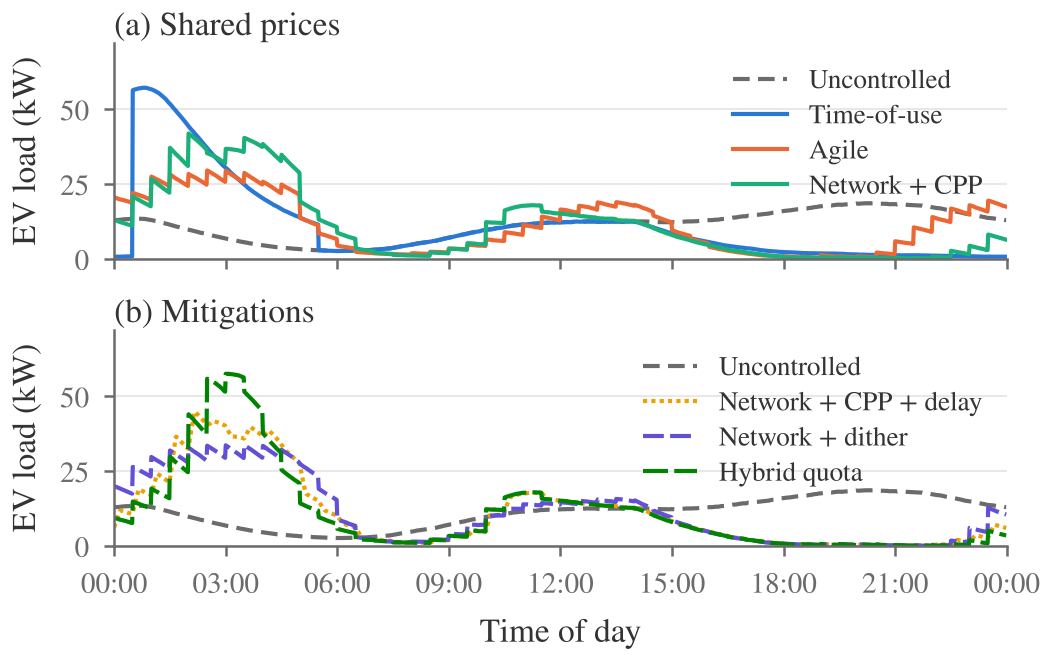
\includegraphics[width=\columnwidth]{f3_profiles}
\caption{Mean EV load over 2000 days, 80\% EV ownership, all chargers smart.
(a) Shared day-ahead prices. (b) Mitigations.}
\label{fig:profiles}
\end{figure}

Fig.~\ref{fig:profiles}(a) confirms that the day in Fig.~\ref{fig:problem}
is typical: every shared price packs the evening charging into a few
overnight half-hours. How much this matters depends on the share of smart chargers
(Fig.~\ref{fig:smartshare}). When half the chargers are smart, shared prices
work well: the share of days over the limit falls from 24.7\% to
6.4--7.8\%, because smart and legacy chargers use different hours. As the
smart share rises further, the smart chargers become the problem. With every
charger smart, overload days rise back to 15.5--19.1\%, and $\CVaR_{95}$ rises
to 124--128~kW, above the 122~kW of uncontrolled charging. Shared prices then
give fewer bad days than uncontrolled charging, but the bad days are worse.

\begin{figure}[t]
\centering
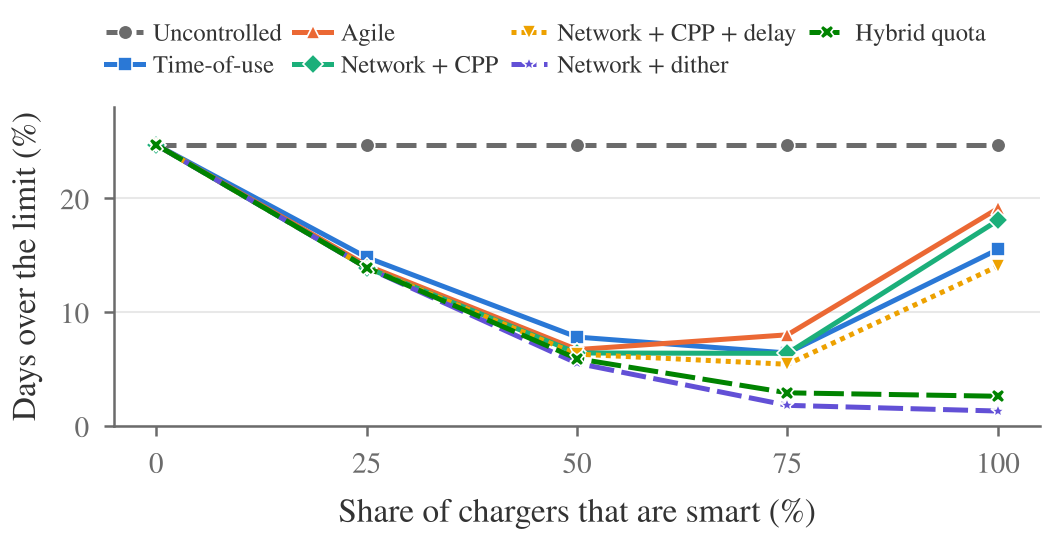
\includegraphics[width=\columnwidth]{f4_smart_share}
\caption{Days over the firm limit against the share of smart chargers, 80\%
EV ownership, 1000 days.}
\label{fig:smartshare}
\end{figure}

\subsection{The surcharge does not settle and causes rebound}
\label{sec:cpp}

With few smart chargers, the CPP fixed point of \cite{gupta2027} settles.
At 80\% ownership and a smart share of up to
0.5, at most 1.3 surcharged slots changed per round over the last 10 rounds,
and the EV forecast moved by at most 1.6~kW. With every charger smart, 3.0
slots changed per round and the forecast moved by 14.8~kW, rising to 4.7
slots and 17.4~kW at 100\% ownership: the CPP keeps chasing the demand it
moves. At 100\% ownership the CPP left overload days unchanged (41.5\% with
it, 41.2\% without) but nearly doubled the number of chargers switching on in
the same minute, from 4.7 to 9.0 (Table~\ref{tab:main}).

\subsection{Mitigations}

\begin{table}[t]
\caption{Results with All Chargers Smart, 2000 Days}
\label{tab:main}
\centering
\footnotesize
\setlength{\tabcolsep}{2.4pt}
\begin{tabular}{@{}lrrrrrr@{}}
\toprule
 & \multicolumn{2}{c}{80\% ownership} & \multicolumn{4}{c}{100\% ownership}\\
\cmidrule(lr){2-3}\cmidrule(l){4-7}
Mechanism & Over & $\CVaR_{95}$ & Over & $\CVaR_{95}$ & Sync & Undel.\\
 & (\%) & (kW) & (\%) & (kW) & (ch.) & (\%)\\
\midrule
Uncontrolled & 24.4 & 122 & 37.5 & 129 & 1.1 & 0.00\\
Time-of-use & 15.8 & 125 & 38.1 & 147 & 9.5 & 0.00\\
Agile & 18.6 & 127 & 41.5 & 150 & 8.5 & 0.00\\
Network, no CPP & 18.1 & 128 & 41.2 & 151 & 4.7 & 0.00\\
Network + CPP & 18.3 & 128 & 41.5 & 151 & 9.0 & 0.00\\
\quad + 600 s delay & 14.7 & 124 & 36.3 & 146 & 2.7 & 0.38\\
\quad + 1800 s delay & 14.7 & 124 & 36.7 & 147 & 1.8 & 1.45\\
\quad + dither & 2.0 & 101 & 9.4 & 116 & 5.2 & 0.00\\
Network + dither & 2.0 & 101 & 7.0 & 113 & 4.1 & 0.00\\
Quota (ASAP) & 7.2 & 106 & 8.6 & 107 & 1.1 & 0.05\\
Hybrid quota & 2.7 & 101 & 5.5 & 102 & 4.2 & 0.29\\
\bottomrule
\end{tabular}\\[2pt]
\begin{minipage}{\columnwidth}\footnotesize
Over: days over the 100.9~kW limit. Sync: most chargers switching on in the
same minute (daily mean). Undel.: energy not delivered by departure. Indented
rows add a mitigation to Network + CPP.
\end{minipage}
\end{table}

\emph{Random delay.} Table~\ref{tab:main} compares the mitigations. The
600~s delay cut synchronised switch-ons at 100\%
ownership from 9.0 to 2.7 chargers, as intended. But the cable heats with the
load over the whole half-hour, and a few minutes' delay leaves the chargers
in the same half-hour, so 36.3\% of days still exceeded the limit (between
28.9\% and 39.2\% across the last 10 CPP rounds). Raising the delay to
1800~s did not help and left 1.45\% of energy undelivered.

\emph{Price dither.} A small offset is enough, because the cheapest half-hours
of the network price differ by less than 0.5\pkwh: a $\pm$2\pkwh{} offset
changes which one is cheapest for each household. It cut overload days to
2.0\% at 80\% ownership and 7.0\% at 100\%, with all energy delivered
(Fig.~\ref{fig:profiles}(b)). Adding the CPP back made the dither less
effective on average (9.4\%) and much less effective in some rounds
(19.3\%), because a 25\pkwh{} surcharge outweighs a 2\pkwh{} offset. Because
chargers pick hours where their own offset is negative, the average price
paid fell from 8.75 to 8.34\pkwh; adding this difference to every price
restores revenue without changing any schedule.

\emph{Quota.} A cap on EV power keeps the worst days near the limit however
the chargers behave, because no half-hour can be booked beyond its capacity.
Booking in price order (the hybrid) gave 5.5\% overload days and a
$\CVaR_{95}$ of 102~kW at 100\% ownership, against 8.6\% and 107~kW when
booking as soon as possible. The ASAP quota does worse because it fills the
evening first, when headroom is smallest and a forecast error is most likely
to cause an overload. The cost is service: the hybrid left 0.29\% of energy
undelivered.

\subsection{Does the charger's algorithm matter?}

\begin{table}[t]
\caption{Days Over the Limit (\%) by Charger Scheduler, 100\% Ownership,
All Chargers Smart, 1000 Days}
\label{tab:sched}
\centering
\footnotesize
\setlength{\tabcolsep}{5pt}
\begin{tabular}{@{}lrrr@{}}
\toprule
Price & Eq.~\eqref{eq:smart} & Commercial & Mixed\\
\midrule
Uncontrolled & \multicolumn{3}{c}{37.8}\\
Time-of-use & 40.0 & 41.6 & 17.0\\
Agile & 44.0 & 40.1 & 36.3\\
Network, no CPP & 43.4 & 42.1 & 38.2\\
Network + CPP & 43.6 & 42.4 & 37.2\\
Network + dither $\pm$2 & 6.3 & 13.3 & 9.0\\
Network + dither $\pm$5 & 3.7 & 6.2 & 4.0\\
\bottomrule
\end{tabular}
\end{table}

Table~\ref{tab:sched} repeats the comparison with the commercial scheduler
and the mixed fleet. The commercial scheduler herds just as much: every
shared price exceeds the limit on 40.1--42.4\% of days, against
37.8\% for uncontrolled charging, and the CPP still raises the number of
chargers switching on in the same minute from 3.5 to
8.9. A mixed fleet helps the ToU tariff (17.0\%), because
its long flat window lets the two schedulers break ties at opposite ends. It
barely helps the network price (37.2--38.2\%), because every half-hour has
a different price, so both schedulers choose the same ones. By removing ties,
a network-aware price also removes the variety that different vendors would
otherwise provide. The dither still works with the commercial scheduler, but
needs to be larger: $\pm$2\pkwh{} gives 13.3\% and $\pm$5\pkwh{} gives
6.2\%.

\subsection{Choosing a mitigation}

Fig.~\ref{fig:penetration} shows how the worst days grow with EV ownership.
Shared prices beat uncontrolled charging up to 60\% ownership and lose beyond
it, reaching a $\CVaR_{95}$ of 145--149~kW at 100\%, against 130~kW. The
dithered network price stays within 1~kW of the firm limit up to 80\%
ownership, with no quota and all energy delivered. Beyond that, only the
hybrid quota stays near the limit (103~kW at 100\%).

\begin{figure}[t]
\centering
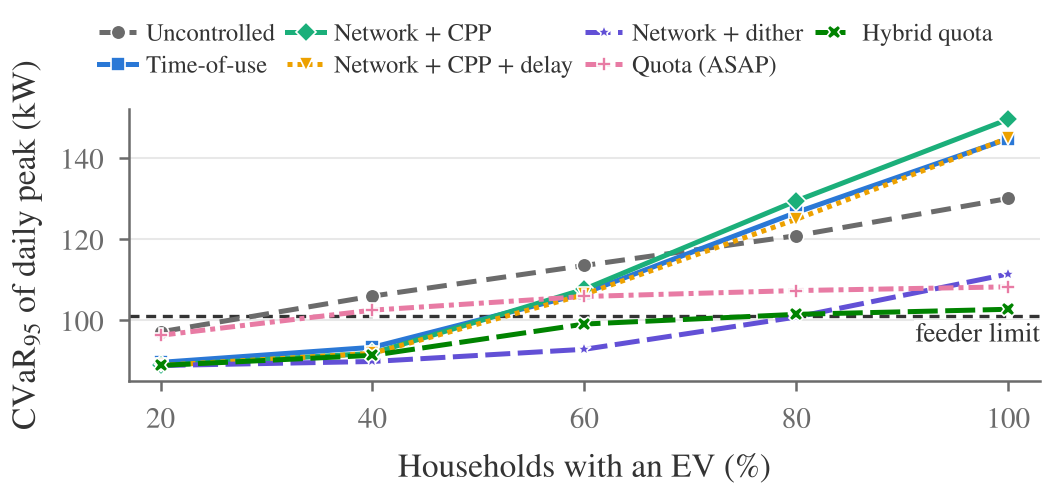
\includegraphics[width=\columnwidth]{f5_penetration}
\caption{$\CVaR_{95}$ of the daily peak against EV ownership, all chargers
smart, 1000 days.}
\label{fig:penetration}
\end{figure}

\begin{figure}[t]
\centering
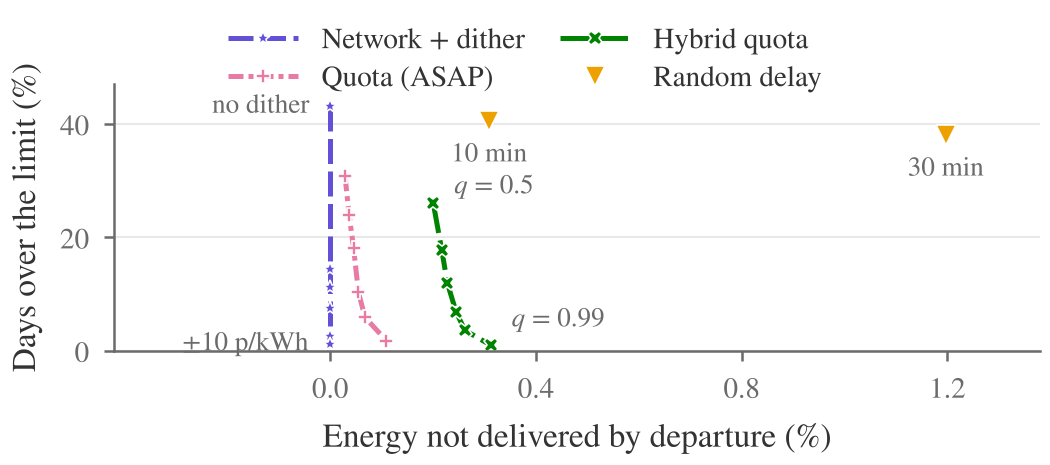
\includegraphics[width=\columnwidth]{f6_tradeoffs}
\caption{Days over the limit against undelivered energy as each mitigation's
setting varies, 100\% EV ownership, all chargers smart, 1000 days. Quota
confidence $q$ runs from 0.5 (top) to 0.99 (bottom); $\delta$ is the dither
half-width.}
\label{fig:frontier}
\end{figure}

Fig.~\ref{fig:frontier} shows each mitigation's trade-off at 100\%
ownership. A larger dither lowers overload days with no loss of service:
2.7\% at $\pm$5\pkwh{} and 1.2\% at $\pm$10\pkwh, at a revenue cost of
1.42\pkwh{} at $\pm$5\pkwh. A more cautious quota ($q$ from 0.5 to 0.99)
cuts the hybrid's overload days from 26.0\% to 1.0\%, while undelivered
energy rises from 0.20\% to 0.31\%. The delay barely helps at any setting.

% ============================================================== CONCLUSIONS
\section{Conclusions}

Smart chargers all read the same price and run similar algorithms, so they
all make the same decision. On the studied London feeder with an EV in every
home, this made every shared price, including the network-aware tariff, worse
than uncontrolled charging on the worst days, stopped the CPP from settling,
and nearly doubled the number of chargers switching on together, also with a
commercial scheduler. The mandated random delay removes the minute-scale
spike but not the half-hourly peak.

Two changes fix this. A slightly different price for each household gives the
chargers different cheapest half-hours, and kept the worst days at the limit
up to 80\% EV ownership with all energy delivered. Above that, only a quota
filled in network-price order kept the worst days near the limit, leaving
under 0.3\% of energy undelivered. A supplier can apply a dither to chargers
already installed; a quota needs the network operator to tell each charger
how much power it may use. This method can be applied to other feeders by
substituting the relevant local parameters, such as travel data, household
demand and feeder ratings, giving network operators a practical way to test a
tariff against smart chargers before it is introduced.

\section*{Acknowledgment}
This research was funded by the Laidlaw Foundation through a Laidlaw
Scholarship. The author thanks Zohaib Akhtar for his guidance throughout this
work, and Yogi Agrawal, Swati Gupta, Vinay Gupta and Tanishka Gupta for their
support.

% ============================================================== REFERENCES
\begin{thebibliography}{00}

\bibitem{gupta2027} A. Gupta and Z. Akhtar, ``Network-aware dynamic pricing for
EV charging on low-voltage networks,'' poster, \emph{F1000Research} (Laidlaw
Scholars Gateway), Taylor \& Francis, 2027, accepted for publication. Code:
\url{https://github.com/RISKMASTER16/network-evpricing}

\bibitem{crozier2020} C. Crozier, T. Morstyn, and M. McCulloch, ``The
opportunity for smart charging to mitigate the impact of electric vehicles on
transmission and distribution systems,'' \emph{Applied Energy}, vol. 268,
art. 114973, 2020.

\bibitem{octopus} Octopus Energy, ``Octopus Go'' and ``Agile Octopus'' tariffs, 2026.
[Online]. Available: \url{https://octopus.energy/smart/}

\bibitem{wen} Y. Wen, D. MacKenzie, and D. R. Keith, ``Modeling the charging
choices of battery electric vehicle drivers by using stated preference
data,'' \emph{Transp. Res. Rec.}, vol. 2572, pp. 47--55, 2016.

\bibitem{scpregs} \emph{The Electric Vehicles (Smart Charge Points)
Regulations 2021}, UK Statutory Instrument 2021/1467, regs.~5 and 11.

\bibitem{evenergy} ev.energy, ``Scheduler,'' developer documentation,
\url{https://developers.ev.energy/docs/understanding/scheduler}.

\bibitem{samende2025} C. Samende, A. Akshaya, S. M. Bhagavathy, J. Melone,
R. Snape, and K. Stewart, ``Herding from uncoordinated smart charging of
EVs: A real-life demonstration,'' in \emph{Proc. IEEE PES ISGT Europe},
2025, pp. 1--5.

\bibitem{catapult2025} C. Rowland, ``The emerging EV overnight demand
peak,'' Energy Systems Catapult, 25 Jun. 2025.

\bibitem{hein2026} T. Hein, L. Wagner, A. Bernhard, and F. Ocker,
``Price-optimized EV and heat-pump scheduling can exceed uncoordinated feeder
peaks,'' arXiv:2610.05916, 2026.

\bibitem{flath2016} C. M. Flath and S. Gottwalt, ``Price-based load
coordination revisited: Augmenting open-loop coordination approaches,''
\emph{Business Research}, vol. 9, no. 1, pp. 157--178, 2016.

\bibitem{fani2024} H. Fani, M. U. Hashmi, E. J. Palacios-Garcia, and
G. Deconinck, ``Impact of dynamic operating envelopes on distribution network
hosting capacity for electric vehicles,'' in \emph{Proc. CIRED 2024 Vienna
Workshop}, IET Conf. Proc., vol. 2024, no. 5, pp. 180--185.

\bibitem{rockafellar2000} R. T. Rockafellar and S. Uryasev, ``Optimization of
conditional value-at-risk,'' \emph{J. Risk}, vol. 2, no. 3, pp. 21--41, 2000.

\bibitem{nts} Department for Transport, ``National Travel Survey: 2024,''
tables NTS0901 and NTS0904.

\bibitem{dftsurvey} Department for Transport, ``Electric vehicle charging
research: Survey with electric vehicle drivers,'' Apr. 2022.

\end{thebibliography}

\end{document}
